\chapter{Implementation}
\label{implementation}

\section{Inspiration and overview}

The project utilises the existing Sophia compiler for the purposes of parsing
and performing the initial type checking, along with decorating abstract syntax
tree with types. The liquid type inference is a side step in the build pipeline
--- it can prevent the code from being passed to the compiler of an intermediate
representation, but it does not provide any input for it\footnote{It does not
  need to be like that, however. Please refer to the discussion,
  \autoref{making_use_of_quals}}.

\begin{figure}[h]
  \caption{Hagia--Sophia compilation pipeline}
  \centering
  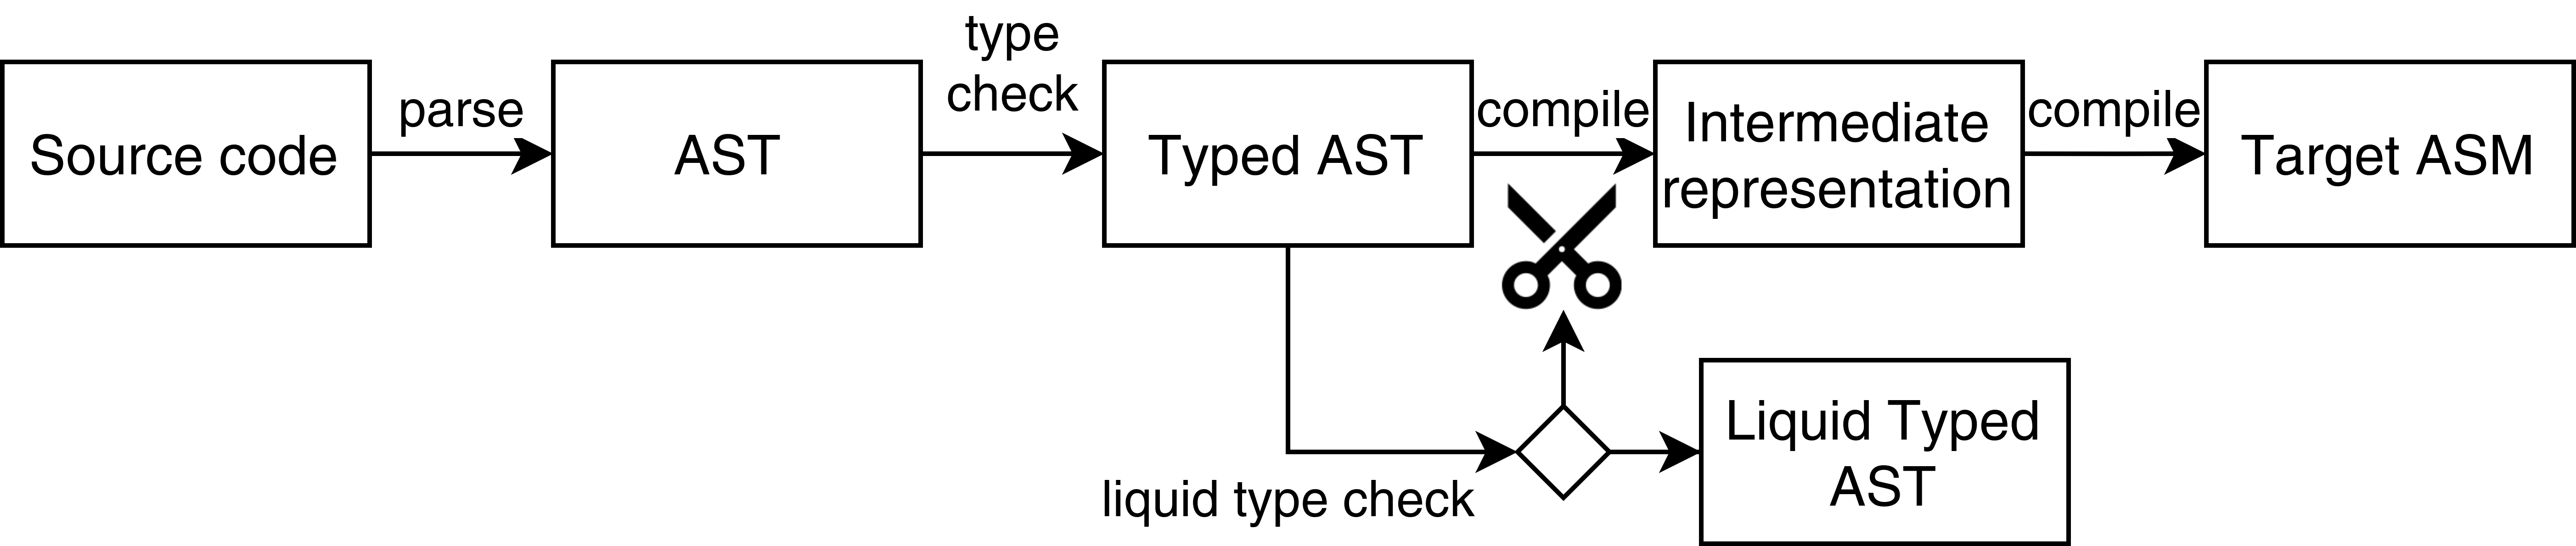
\includegraphics[scale=0.08]{hagia_pipeline}
\end{figure}

The implementation follows the algorithm proposed in Rondon's paper
\cite{liquid}, which is split into three main phases:

\subsubsection{Hindley--Milner type inference}

This step is already done by the Sophia type checker, so its details are not
discussed in this document. What is important, it returns an AST decorated with
type annotations on each node. This information shall serve for the liquid
typing initialisation in the next phase.

\subsubsection{Constraint generation}

The purpose of this process is to upgrade the types inferred in the previous
step to their liquid equivalents, and define constraints that must hold in order
to make the liquid typing valid. The generated constraints reflect dependencies
between types and assert assumptions about the control flow. Some constraints
are fixed, such as these explicitly given by the user, and some are yet unknown
and are subject to the weakening in the next step.

\subsubsection{Constraint solving and iterative weakening}

This is the process of satisfying the constraints. They are iteratively checked
for validity and if it is not the case, the inference relaxes the ones that can
be adjusted, until the system is consistent. If it manages to converge to a
point where every constraint is satisfied, a liquid typing is returned.
Otherwise, an error is reported.

\section{Used technology}

As the existing Sophia compiler is written in Erlang, it is most convenient to
use a programming language that also runs on the Open Telecom Platform
\cite{ericssonab2021}. Of such languages, Erlang and Elixir seem to be the most
mature and since the latter requires some additional effort for inter-operating
with the current implementation, the former was chosen.

During constraint solving the help of an SMT solver is invaluable, so following
Rondon's implementation of liquid types, Z3 by Microsoft Research
\cite{10.1007/978-3-540-78800-3_24} was chosen. Among many of its advantages,
the most convincing is the support of the SMT-lib language and a wide variety of
theories and abstractions that are useful for expressing judgements about the
values in Sophia. Furthermore, its performance has been proven to excel by
numerous successes at SMT-COMP competitions.

\section{Preprocessing}

Before the main algorithm is executed, the AST needs to be stripped of certain
abstractions. This is mostly due to the fact that the solving utility accepts
only a tight range of expressions, and it is much more convenient to analyse
simpler code and in a more selective manner. Therefore, several preprocessing
techniques are introduced.

\subsection{$\alpha$-normalisation}

\begin{defi}
  An expression is in the $\alpha$-normal form if it has no subexpressions that
  introduce variables which are already bound in their context.
\end{defi}

$\alpha$-normalisation is therefore a process of elimination of variable
shadowing. It can be done by performing subsequent $\alpha$-conversions
\cite{alpha_norm}, although in Hagia an error is thrown if a name collision is
detected. This is because shadowing can lead to hard to detect bugs if both
variables have the same type.

Without this process certain dependencies would become malformed or impossible
to express. Consider the following code:

\begin{minipage}{\linewidth}
\begin{lstlisting}[language=sophia]
let x = 1
let x = x + x  // this is not recursive
x
\end{lstlisting}
\end{minipage}

There is a collision on $x$ which can effectively confuse the solver; it would
receive an assertion that $x = 1 \land x = x + x$ which is not satisfiable. In
fact, the former $x$ and the latter one are different variables and thus have to
be reffered with different names. $\alpha$-normalisation is there to fix it by
appriopriate renaming:

\begin{minipage}{\linewidth}
\begin{lstlisting}[language=sophia]
let x_0 = 1
let x_1 = x_0 + x_0
x_1
\end{lstlisting}
\end{minipage}

\subsection{A-normalisation}

A-normalisation simplifies code by unpacking certain compound expressions and
explicitly assigning their parts to variables \cite{10.1145/173262.155113}. Most
often, its purpose is to reduce the gap between high-level abstract programs and
their lower-level representations. An accurate definition has been proposed by
Matt Might in one of his articles \cite{a_norm}:

\begin{quote}
  \begin{defi}
    An expression is atomic if:

    \begin{itemize}
    \item it is guaranteed to terminate;
    \item it causes no side effects;
    \item it causes no control effects; and
    \item it never produces an error.
    \end{itemize}
  \end{defi}

  \begin{defi}
    In A-Normal Form, all non-atomic (complex) expressions must be let-bound, or
    else appear in tail position.
  \end{defi}
\end{quote}

For instance, the following code

\begin{minipage}{\linewidth}
\begin{lstlisting}[language=sophia]
function factorial(n) =
  if(n == 0) 1
  else factorial(n - 1) * n
\end{lstlisting}
\end{minipage}

would be converted to

\begin{minipage}{\linewidth}
\begin{lstlisting}[language=sophia]
function factorial(n) =
  let b = n == 0
  if(b) 1
  else
    let v1 = n - 1
    let v2 = factorial(v1)
    v2 * n
\end{lstlisting}
\end{minipage}

Code in this form is much more convenient to analyse because every non-jumping
intermediate expression is named. This provides the refiner with handles to all
necessary parts of the program, allowing it to refer them independently. The
semantics are entirely preserved during A-normalisation.

\subsection{Purification}

This step is unavoidable due to the impure nature of Sophia, which does not
weave into Rondon's algorithm very well. Furthermore, mutable state is not
supported by the purely declarative SMT solver language. As stated in the
\autoref{chapter_sophia}, smart contracts do process an explicit mutable state
along with some additional variable properties like balances, remaining gas and
so on. This applies not only to the main contract, but also remote ones. Thus,
the aim is to convert the code to an equivalent one which is free of these
mechanisms.

Purification is the most convenient to perform on already A-normalised code due
to the assumption of purity of all sub-expressions in non-tail positions. This
vastly reduces the cases to cover, as it is no longer needed to check if, for
example, arguments in a function application interfere with the state. The
process does not need to preserve the A-normal form though. Since the
A-normalisation process does not affect the purity, it can be triggered once
again after the purification.

The expected outcome should resemble the \texttt{State} monad
\cite{markp.jones1995} pattern, where each function is additionally
parameterised by an argument representing the incoming state of computation and,
if it is stateful, modified to return the new state aside from the original
result. A similar approach is applied to the built-in statements that are
identified to be impure. This way the system keeps track of the changes by
making subsequent stateful operations introduce new variables representing
different stages of the chain state.

For the purpose of this algorithm the \texttt{chain\_state} is introduced. It
encapsulates everything related to the blockchain that might be altered during
the execution. In the current implementation, it is limited to two variables:

\begin{itemize}
\item \texttt{state} --- for tracking the internal state of the contract
\item \texttt{balance} --- for tracking the balance of the contract
\end{itemize}

This list can be further extended, if there is a need for a more detailed view
on the interaction with the chain. For convenience, handles of these values can
be stored in a dedicated \texttt{record} type and passed along with the control
flow. Although, Hagia keeps them separated to simplify the process of constraint
generation.

The purification process is itself stateful as it needs to keep the most actual
state reference and update it as needed. In case of Sophia, there are actually
not many primitive operations which are impure; thanks to the A-normalisation,
the only cases that are needed to be treated specially are:

\begin{itemize}
\item \texttt{state} --- should be replaced with the variable representing the
  current state reference.
\item \texttt{put} --- replaced with \texttt{()} and the state reference is set
  to the argument.
\item \texttt{Chain.spend} --- sets the balance variable to the previous one
  reduced by the sent amount. The expression has to be again typed as a
  non-negative integer.
\item \texttt{Contract.balance} --- replaced with the balance variable.
\item Remote contract calls --- the function call should be kept so the return
  value can be computed (possibly with an updated liquid type of
  \texttt{Call.value}, if the refinement system handles it). If the call value
  is set, then it should be subtracted from the balance before the call,
  similarly to the \texttt{Chain.spend}. Furthermore, the initial balance of the
  called contract can be safely assumed to be greater or equal to the sent
  value.
\item Stateful function calls --- since they may modify the state, they should
  return a tuple with the updated state and the actual return value.
\item Calls by a variable --- there is no control if the underlying function is
  stateful or not, so it is better to assume it is.
\item Calls to higher order functions --- if there is an argument which may be a
  stateful function, then the higher-order function should be considered
  stateful as well.
\item Oracle and AENS specific utilities --- if these object can be subjects of
  refinement, they should be handled appropriately. Current implementation of
  Hagia does not consider them, however.
\end{itemize}


The resulting code should be entirely pure and independent of these operations.
The semantics shall be preserved only in the purely computational sense --- the
outcome shall not be actually suited to interact with the blockchain, but rather
represent a more high-level view on the execution.
\autoref{example_before_purification} and \autoref{example_after_purification}
present examples of code before and after purification, respectively.

\begin{code}[h]{lexers/sophia.py:SophiaLexer -x}{Code before purification}{example_before_purification}
type state = int

stateful entrypoint f : () => address
entrypoint g : int => int

stateful entrypoint example(amount : int) : int =
  let addr = f()
  Chain.spend(addr, amount)
  put(amount)
  g(Chain.balance)
\end{code}

\begin{code}[h]{lexers/sophia.py:SophiaLexer -x}{Code after purification}{example_after_purification}
record chain_state =
  { state    : int,
    balance  : {b : int | b >= 0} }

entrypoint f : (chain_state) => chain_state * address
entrypoint g : (chain_state, int) => int

entrypoint example(cs0 : chain_state, amount : int) : chain_state * int =
  let (cs1, addr) = f(cs0)
  let cs2 = cs1{balance = cs1.balance - amount}
  let cs3 = cs2{state = amount}
  (cs3, g(cs3, cs3.balance))
\end{code}

In the examples, the stateful entrypoint \texttt{f} has been extended with an
additional argument carrying the representation of the incoming chain state and
modified to return the updated version of it. On the other hand, while
\texttt{g} also receives the chain state, its return value remains the same,
because it is not stateful. The call to \texttt{f} updates the carried chain
state reference aside from assigning the original result value to the
\texttt{addr} variable. The further calls to \texttt{Chain.spend}, \texttt{put}
and \texttt{Chain.balance} behave accordingly.

\section{The $\Gamma^*$ environment}

The $\Gamma^*$ environment has been defined as an extension to the regular
$\Gamma$ environment by changing base types into their liquid equivalents, and
attaching an additional path predicate. In Hagia, however, there are some
further features arising from the properties of Sophia. Among them there are
scope handles, current namespace and a registry of stateful entrypoints.
Moreover, for the purpose of the initial assignment algorithm described in the
\autoref{initial_assignment}, a collection of potentially relevant integers is
stored.

\section{Constraint generation}

This phase does not perform any verification itself, but rather defines a number
of statements that must hold in certain environments. Aside from that, it is
similar to the regular type checking as it computes a liquid typing for the
provided typed AST.

There are four kinds of such constraints:
\begin{itemize}
\item \emph{Well-formed} constraint which indicates existence of a liquid type,
  ensuring that it is properly initialised and the assigned qualifiers are
  correctly typed in a given environment. Denoted by $\Gamma^* \vdash \tau$
  where $\Gamma^*$ is the environment and $\tau$ is a well-formed type.
\item \emph{Subtype} constraint which asserts that some type is a subtype of
  another in a certain environment. Described using $\Gamma^* \vdash \tau_{sub}
  <: \tau_{sup}$ meaning that $\tau_{sub}$ is a subtype of $\tau_{sup}$ in
  $\Gamma^*$.
\item \emph{Reachable} constraint which ensures that some environment has a
  chance of being visited.
\item \emph{Unreachable} constraint which indicates an invalid environment which
  must be proven never to occur.
\end{itemize}

Each of these describe certain promises that have to be fulfilled in order to
find a valid liquid typing. This section reviews the process of generating them
from a typed AST.

\subsection{Decorating types with logical qualifiers}

This operation turns a base type into a corresponding liquid one. As provided by
the syntax, the user can specify liquid types manually and these remain
unchanged. Otherwise, if a non-liquid type is detected, it is enhanced with an
appropriate refinement. Fresh predicates created in this phase are represented
by \emph{liquid templates} as described in Rondon's algorithm \cite{liquid}. A
liquid template consists of a \emph{liquid type variable} and a \emph{pending
  substitution}. The former serves as the identifier of a predicate to be
resolved. Each time a substitution is applied to a liquid template, it is
accumulated in the pending substitution instead of altering the underlying
predicate, so it will not affect other occurences of that type.

Since the aim is to infer as strong judgements as possible, the positions of
types must be taken into account during the initialisation. When a type
describes the output of some computation, like for example the result of a
function or a variable introduction, it is called \emph{covariant}. It should
receive the whole space of possible qualifications and be therefore decorated
with a fresh liquid template. Otherwise, if a type is on an input position, such
as a function argument or a map key, it is defined to be \emph{contravariant}.
In contrary to the covariant ones, these types receive empty qualifications
which put no restrictions on the inhabiting values. Consequently, simple types
are decorated as follows:

\begin{lstlisting}[language=pseudocode]
fresh_template(variance) =
    let predicate =
            if variance == Covariant then fresh_liquid_var()
            else $\top$
        subst = []
    return make_template(subst, predicate)

fresh_liquid_simple(variance, $\mathbb{T}$) = -- covers primitives and type vars
    return $\{\nu : \mathbb{T} | \text{fresh\_template(covariant)}\}$
\end{lstlisting}

More than that, the variance switches each time an input position is entered, so
an argument of a function which is an argument of a higher-order function shall
be covariant instead.

\begin{lstlisting}[language=pseudocode]
switch_variance(Covariant) = Contravariant
switch_vairance(Contravariant) = Covariant

fresh_liquid_fun(variance, args, ret) =
    let args1 = [ ($\{\text{arg} : \text{fresh\_liquid}(\text{switch\_variance(variance)}, \tau)\}$)
                | $\{\text{arg} : \tau\}$ $\leftarrow$ args]
        ret1 = fresh_liquid(variance, ret)
    return $\text{args1} \to \text{ret1}$
\end{lstlisting}

The intuition here is to start with the least possible knowledge, while leaving
an opportunity for learning new facts. Covariant types describe values that are
built up across the computation, so in order to represent full uncertainty the
refiner considers all possible properties which may or may not apply. In
contrast, there is no judgement to be put on the incoming values, as they do not
depend on the expression itself, but rather on its use in other contexts.
Because of this, the refiner must be prepared to receive anything in their place
and thus strip all the assumptions off.

The only exception to this rule are lists' length predicates, because one can be
always sure that they will never be negative. In this special case, they are
initialised to $\{\nu : \texttt{list(\_)} | \nu \geq 0\}$.

\begin{lstlisting}[language=pseudocode]
fresh_liquid_list(variance, elem_t) =
    let len_predicate =
            if variance == Covariant then fresh_liquid_var()
            else $\nu \geq 0$
        subst = []
        elem_lt = fresh_liquid(variance, elem_t)
    return $\{\nu : \text{list(elem\_lt)} | \text{make\_template(subst, len\_predicate)}\}$
\end{lstlisting}

\subsubsection{Example}

For a reference of what happens in this process, let us consider the type of the
\texttt{List.map} function from the standard library, that applies a function
over every element of a given list. Assuming that a function is the first
argument, the type inferred by the original type checker is $(\alpha \to \beta,
\texttt{list}(\alpha)) \to \texttt{list}(\beta)$, which after decoration is
changed to

$$(\{\texttt{x} : \alpha | \rho_1\} \to \{\nu : \beta | \top\},
\{\texttt{l} : \texttt{list}(\{\nu : \alpha | \top\}) | \texttt{l} \geq 0\}\})
\to \{\nu : \texttt{list}(\{\nu : \alpha | \rho_2\}) | \rho_3\}$$

Where $\rho_1$, $\rho_2$ and $\rho_3$ are fresh liquid templates and $\top$ is an
empty predicate. The return value of the incoming function has been initialised
with an empty predicate, because it is on a contravariant position. A similar
thing has happened to the input list and its elements, except that non-negative
length has been assumed. The argument of that function is back on a covariant
position, so, just like the return value of \texttt{List.map}, has received a
fresh liquid template. In the end, $\rho_1$ and $\rho_2$ are resolved to $\top$,
and $\rho_3$ turns into $\nu = l$ to express that \texttt{List.map} preserves
the length. If the programmer had specified the predicates under the liquid
templates explicitly, they would have been left unaltered.

\subsubsection{User-definable types}
\label{user_definable_types}

Type aliases are resolved and processed further down.

\begin{lstlisting}[language=pseudocode]
fresh_liquid_alias(variance, name) =
    return fresh_liquid(variance, solve_name(name))
\end{lstlisting}

The identifiers of records are expanded to expose their underlying definitions
and turned into their liquid equivalents.

\begin{lstlisting}[language=pseudocode]
fresh_liquid_record(variance, $\mathbb{T}$) =
    let fields1 = [($\text{field} : \text{fresh\_liquid}(\text{variance}, \tau)$) | ($\text{field} : \tau$) $\leftarrow$ $\mathbb{T}$.fields]
    return $\{\mathbb{T} <: \text{fields1}\}$
\end{lstlisting}

Variants are unfolded similarly to records, but there is one more thing specific
them; their user-facing representation follows the description specified in
\autoref{liquid_types}, but for constraint generation they need to be
preprocessed to simplify the splitting rules discussed in the
\autoref{sub:constraint_splitting}. As stated before, liquid variants restrict
their domains not only by using liquid types in parameters of constructors, but
also allow banishing whole constructors from defining the inhabiting values,
regardless of their arguments. In this phase these two roles are split by
redefining liquid variants to utilise all their constructors and keep separate
\emph{tag predicates} that assert that a given value may or may not have been
created using given constructor.

\begin{lstlisting}[language=pseudocode]
fresh_liquid_variant(variance, $\mathbb{T}$) =
    let constructors1 =
            [ constr([($\{\text{arg} : \text{fresh\_liquid}(\text{variance}, \tau)\}$) | $\{\text{arg} : \tau\}$ $\leftarrow$ args])
            | constr(args) $\leftarrow$ $\mathbb{T}$.constructors]
    return $\{\{\nu : \mathbb{T} | \text{fresh\_template(variance)}\} <: \text{constructors1}\}$
\end{lstlisting}

Tag predicates take form of a conjunction of (possibly negated) either equality
against nullary constructors or existential expressions stating that it is
possible to find such arguments, that applied to that constructor build a
well-typed value. Although Sophia does not support existential quantification,
these qualifications do not escape internals of the inference algorithm, so they
do not conflict with the syntax.

More than that, missing constructors in user-defined liquid variants have
their parameters restricted to their minimal subtypes. It essentially means that
each covariant argument is initialised with a single qualification $\bot$
(\texttt{false}) instead of a fresh template. This allows expressing subtyping
more accurately later on.

\begin{minipage}{\linewidth}
\begin{lstlisting}[language=pseudocode]
fresh_liquid_dep_variant(variance, $\mathbb{T}$, declared_constructors) =
    let all_constructors = $\mathbb{T}$.constructors
        names_declared = [constr | constr(args) $\leftarrow$ declared_constructors]
        names_all      = [constr | constr(args) $\leftarrow$ all_constructors]

        constructors_combined =
            [constr(args) | constr(args) $\leftarrow$ declared_constructors] +
            [constr(args) | constr(args) $\leftarrow$ all_constructors,
                            $\text{constr} \notin \text{names\_declared}$]

        constructors1 =
            [ constr([($\{\text{arg} : \text{fresh\_liquid}(\text{variance}, \tau)\}$) | $\{\text{arg} : \tau\}$ $\leftarrow$ args])
            | constr(args) $\leftarrow$ constructors_combined]
        is_not(constr, arity) =
            if arity == 0 then return $\nu \neq  \text{constr}$
            else return $\lnot(\exists \text{args}. \nu = \text{constr(*args)})$
        tag_pred =
            fold_left(($\land$), $\top$,
                [ is_not(constr, length(args))
                | constr(args) $\leftarrow$ all_constructors,
                  $\text{constr} \notin \text{names\_declared}$])

    return $\{\{\nu : \mathbb{T} | \text{tag\_pred}\} <: \text{constructors1}\}$
\end{lstlisting}
\end{minipage}

For example, let us consider a type defined as \texttt{datatype t = C1 | C2(int)
  | C3(int)} and its liquid subtype $\{\texttt{t} <: \texttt{C2}(\{\nu :
\texttt{int} | \nu > 0\})\}$. After decoration, it is restructured to
$$\{\{\nu : \texttt{t} | \nu \neq \texttt{C1} \land \lnot(\exists a_1. \nu =
\texttt{C3}(a_1))\} <: \texttt{C1} | \texttt{C2}(\{\nu : \texttt{int} | \nu >
0\}) | \texttt{C3}(\{\nu : \texttt{int} | \bot\})\}$$

That reads: ``a type of such $\nu : \texttt{t}$, that $\nu$ is not \texttt{C1}
nor can be constructed with \texttt{C3}, and if it is built with \texttt{C2}
then its parameter is greater than zero''. While being more complicated, it
explicitly describes the meaning of the former notation. Furthermore, the
falsified assumption on the parameter of \texttt{C3} causes the type
$\{\texttt{t} <: \texttt{C2}(\{\nu : \texttt{int} | \nu > 0\})\}$ to be a
subtype of $\{\texttt{t} <: \texttt{C2}(\{\nu : \texttt{int} | \nu > 0\}) |
\texttt{C3}(\{\nu : \texttt{int} | \bot\})\}$. Note that because of the tag
predicate the subtyping does not work the other way around --- please refer to
the \autoref{effective_variant_types} for the discussion.

\subsection{Preparing the environment}

Normally namespaces and contracts are processed in a way that allows mutual
recursion among the functions they contain, but not across the scopes. This does
not necessarily reflect the case of liquid inference, as the dependencies may
flow in both directions. Thus, before the functions' bodies are examined, all
signatures are refined and registered in the environment. Custom type
definitions have to be handled beforehand.

An important requirement that needs to be verified in this step is that no
entrypoint has assumptions on its input. This is crucial when user decides to
declare liquid types on their own, because none of the contravariant assertions
would actually be checked at runtime. Subsequently, the programmer might be
wrongfully convinced that the function is safe from receiving improper input.

Formally speaking, in all entrypoints' signatures, the contravariant types must
not be qualified by any logical statements that would exceed the guarantees made
by the virtual machine. The covariant ones are free of this restriction, because
they serve as ``promises'' of the contract, not ``expectations''. Note that
despite being theoretically an input of every function, the \texttt{state} value
always comes from inside of a contract and cannot be therefore set out-of-domain
by a malicious user. Because of that, it should be considered solely covariant
in this context.

\subsection{Constraining global functions}

For a given function $f$ we define its \emph{global type} $F_g$ derived from the
previous step, and its \emph{local type} $F_l$ which emerges from the constraint
generation of its body. The body is processed in the environment $\Gamma^*_a$,
which is extended by the arguments' bindings and the assertions that the
arguments from the definition and the type declaration are in fact the same
values.

Afterwards, appropriate constraints are produced. First, it is necessary to
assert that both $F_l$ and $F_g$ are well-formed. Next, there must be a
subtyping relation between $F_l$ and $F_g$, so the implementation fits the
declaration.

\subsubsection{Example}

For a simplistic example, let us consider a constant function that returns 1.
However, the programmer has specified its type just to return an integer that is
greater than 0. The function can be defined as follows:

\begin{minipage}{\linewidth}
\begin{lstlisting}[language=sophia]
function
  pos_int : () => {r : int | r > 0}
  pos_int() = 1
\end{lstlisting}
\end{minipage}

In this snippet, $F_l$ is inferred to be $() \to \{r : \texttt{int} | r =
1\}$ and $F_g$ is declared as $() \to \{r : \texttt{int} | r > 0\}$. The
subtyping relation between these types holds, making the program well-typed.
Details on how $F_l$ has been constructed are discussed in the
\autoref{ssec:constr_expr} in this chapter. The verification of the subtyping is
covered in the \autoref{sec:solving}.

\subsection{Constraining expressions}
\label{ssec:constr_expr}

Since Sophia has a very rich syntax, there are numerous cases to consider in
this step. Because of that, only the most principal, unique, or otherwise
interesting have been selected. Needless to say, many of the omitted cases can
be easily derived from the presented ones. For a broader view, please refer to
the original implementation in the GitHub repository.

\subsubsection{Variables}

Constraining variables depends on whether their type is simple enough to make
the equality assertion meaningful. In the original implementation
\texttt{is\_simple} is defined to check if the type is either a primitive or a
type variable. In such a case, an equality assumption provides as much
information as the current knowledge about the underlying value, but can be
expressed with just a single qualification instead. Otherwise, the original type
is inherited.

\begin{minipage}{\linewidth}
\begin{lstlisting}[language=pseudocode]
constr_expr_var($\Gamma^*$, name, type) =
    let ltype = fresh_liquid($\Gamma^*$, type)  -- solves aliases by the way
        baseT = base_type(ltype)  -- `type` is not guaranteed to be base
    if is_simple(baseT) then
        return $\{\nu : \text{type} | \nu = \text{name}\}$
    else
        return type_of($\Gamma^*$, name)
\end{lstlisting}
\end{minipage}

\subsubsection{Integer arithmetic}
\label{constr_expr_int}

The integer literal is one of the simplest cases, because every property of it
can be concluded directly from its known value.

\begin{lstlisting}[language=pseudocode]
constr_expr_int($\Gamma^*$, n) =
    return $\{\nu : \text{int} | \nu = \text{n}\}$
\end{lstlisting}

The arithmetic operations are typed in a way that allows the solver deriving the
information about their result directly from the operands. As an example, the
division has been chosen because it presents an additional requirement for the
right-hand value not being equal to 0.

\begin{lstlisting}[language=pseudocode]
constr_expr_op($\Gamma^*$, "/") =
    let opLV  = fresh_id()
        opRV  = fresh_id()
    return $(\{\text{opLV} : \text{int}\}, \{\text{opRV} : \text{int} | \text{opRV} \neq 0\}) \to \{\nu : \text{int} | \nu = \text{opLV} / \text{opRV}\}$
\end{lstlisting}

\subsubsection{Function application}

In Hindley--Milner, the type of a function application is inferred to be its
codomain. However, with liquid types it may vary depending on the values of the
arguments. Consequently, an appropriate substitution has to be applied. It can
be done directly due to the A-normalisation, which ensures that the arguments
are atomic and thus simple enough to be used in qualifiers. In order to ensure
that the application is valid, a proper subtyping relation must hold between the
declared and provided arguments. Therefore, for each pair $(a_i, \tau_i)$, where
$\tau_i$ is the type of the i-th argument from the function domain and $a_i$ is
the inferred type of the respective value, the $\Gamma^* \vdash a_i <: \tau_i$
constraint is produced.

\begin{lstlisting}[language=pseudocode]
constr_expr_app($\Gamma^*$, fun, argsApp) =
    let (argsFT $\to$ retT) = constr_expr($\Gamma^*$, fun)
        argsT = constr_exprs($\Gamma^*$, argsApp)
        argsSubst =
          [(argName, argVal) | ($\{\text{argName} : \_\}$, argVal) $\leftarrow$ zip(argsFT, argsApp)]

    for ($\{\_ : \text{argT}_\}$, argFT) in zip(argsT, argsFT) do
        constraint($\Gamma^* \vdash \text{argT} <: \text{argFT}$)
    return apply_subst(argsSubst, retT)
\end{lstlisting}

For example, considering an expression \texttt{4 / 2}, the system shall infer
the type $\{\nu : \texttt{int} | \nu = 4 / 2\}$ and generate the following
constraints:

\begin{align*}
  & \Gamma^* \vdash \{\nu : \texttt{int} | \nu = 4\} <: \{\nu : \texttt{int}\}\\
  & \Gamma^* \vdash \{\nu : \texttt{int} | \nu = 2\} <: \{\nu : \texttt{int} | \nu \neq 0\}
\end{align*}

While the first one does not introduce any useful information, the latter
asserts that there is no division by zero. Although the presented case is rather
trivial, this requirement would bring a lot of value if the right-hand operand
was a variable.

\subsubsection{\texttt{if} expression}

The \texttt{if} expression is one of the most representative examples of the
path predicate in use. First, the condition is processed, but only for the
purpose of constraints generation, as the type is already known to be boolean.
Then, the positive and negative cases are considered in $\Gamma^*$ with the path
predicate extended by the respective valuations of \texttt{cond} (the
\texttt{assert} function). In the end, the final type must be a supertype of
what has been inferred for both branches. The reachability constraints are
included to forbid dead code.

\begin{lstlisting}[language=pseudocode]
constr_expr_if($\Gamma^*$, cond, thenEx, elseEx, type) =
    constr_expr($\Gamma^*$, cond)
    let $\Gamma^*_t$ = assert(cond, $\Gamma^*$)
        $\Gamma^*_e$ = assert($\lnot$cond, $\Gamma^*$)
        thenT = constr_expr($\Gamma^*_t$, thenEx)
        elseT = constr_expr($\Gamma^*_e$, elseEx)
        $\tau$ = fresh_liquid($\Gamma^*$, type),
    constraint($\Gamma^* \vdash \tau$)
    constraint(reachable($\Gamma^*_t$))
    constraint(reachable($\Gamma^*_e$))
    constraint($\Gamma^*_t \vdash \text{thenT} <: \tau$)
    constraint($\Gamma^*_e \vdash \text{elseT} <: \tau$)
    return $\tau$
\end{lstlisting}

\subsubsection{Pattern matching}

Pattern matching is not covered in Rondon's work, so it is explained in more
details here. The very first step is to extract constraints from the desctructed
expression (the \texttt{switched} variable).

\begin{lstlisting}[language=pseudocode]
constr_expr_switch($\Gamma^*$, switched, alts, type) =
    let switchedT = constr_expr($\Gamma^*$, switched),
        $\tau$ = fresh_liquid($\Gamma^*$, type)
    constr_cases($\Gamma^*$, switched, switchedT, $\tau$, alts)
    constraint($\Gamma^* \vdash \tau$)
    return $\tau$
\end{lstlisting}

The alternatives are processed and combined into the return type similarly to
\texttt{if} branches, with the difference of using more advanced conditions,
additionally capable of introducing variables. Each alternative has its body
processed in the environment of a successful match to the current pattern along
with an assumption of failing matches in previous cases, as \texttt{switch}
considers the clauses top--down. An additional reachability constraint is
generated in order to disallow dead code. At the end, where no further
alternatives are available, the environment is asserted to be unreachable by a
relevant constraint. This prevents a pattern-exhaustion error and enforces the
programmer to consider all possible cases.

\begin{lstlisting}[language=pseudocode]
constr_cases($\Gamma^*$, switched, switchedT, returnT, alts) =
    if alts.non_empty() then
        let (pat $\implies$ val) = alts.first()
            ($\Gamma^*_+$, $\Gamma^*_-$) = match_to_pattern($\Gamma^*$, pat, switched, switchedT)
            valT = constr_expr($\Gamma^*_+$, val)
        constraint($\Gamma^*_+ \vdash \text{valT} <: \text{returnT}$)
        constraint(reachable($\Gamma^*_+$))
        constr_cases($\Gamma^*_-$, switched, switchedT, returnT, alts.drop_first())
    else constraint(unreachable($\Gamma^*$))
\end{lstlisting}

The split of the environments is done by the \texttt{match\_to\_pattern}
function. The auxiliary \texttt{match\_to} procedure builds up a predicate
describing a successful match and an environment in which all pattern variables
are bound. With this information, \texttt{match\_to\_pattern} creates a
succeeding environment with the assumptions applied and a failing one with no
new variables, but with the negation of the predicate asserted.

\begin{lstlisting}[language=pseudocode]
match_to_pattern($\Gamma^*$, pat, expr, type) =
    let ($\Gamma^*_m$, pred) = match_to($\Gamma^*$, pat, expr, type, $\top$)
        $\Gamma^*_+$ = assert(pred, $\Gamma^*_m$)
        $\Gamma^*_-$ = assert($\lnot$ pred, $\Gamma^*$)
    return ($\Gamma^*_+$, $\Gamma^*_-$)
\end{lstlisting}

During the predicate build-up there are three main kinds of patterns:
\begin{itemize}
\item Literal patterns --- for example integers. They extend the matching
  predicate by an assumption that the destructed expression has a given
  value.
\item Variables --- these do not add anything to the matching predicate, but
  instead extend the environment with an appropriate variable binding.
\item Complex patterns --- for example tuples or lists. They require unpacking
  the component data and sometimes verifying the general form of the destructed
  value. In case of a tuple, the pattern matching proceeds by matching the
  projections against the respective sub-patterns. In case of variant types, an
  additional constructor tag assertion is added. Lists introduce mock
  \texttt{int} variables which derive their qualifications from length
  predicates and are asserted to imply the value induced by the pattern.
\end{itemize}

It is assumed that \texttt{match\_to} splits over possible kinds of patterns and
dispatches across functions as such:

\begin{minipage}{\linewidth}
\begin{lstlisting}[language=pseudocode]
match_to_var($\Gamma^*$, name, expr, type, pred) =
  return (bind_var(name, type, $\Gamma^*$), pred)

match_to_int($\Gamma^*$, n, expr, type, pred) =
  return ($\Gamma^*$, $\text{expr} = \text{n} \land \text{pred}$)

match_to_tuple($\Gamma^*$, pats, patsT, expr, pred) =
    return fold_left(
      fun(($\Gamma^*_1$, pred_1), (pat, patT, idx)) $\to$
           return match_to_pattern($\Gamma^*_1$, pat, expr[idx], patT, pred_1)
      end,
      ($\Gamma^*$, pred),
      zip(pats, patsT, [1..length(pats)])
    )
\end{lstlisting}
\end{minipage}

To visualise the process, let us consider a simple pattern matching shown in the
code snippet below:

\begin{lstlisting}[language=sophia]
function f(m : option(int)) : int =
  switch(m)
    None => 1
    Some(0) => 1
    Some(n) => n
\end{lstlisting}

The constraints are generated as follows:

\begin{enumerate}
\item First, the destructed expression \texttt{m} comes with a (redundant in
  this case) well-formedness constraint on its type:
  $$\Gamma^* \vdash \texttt{option(int)}$$.
\item The overall return type is declared to be well-formed:
  $$\Gamma^* \vdash \tau$$
\item In the first alternative, \texttt{m} is matched against a 0-arity
  constructor \texttt{None}. Hence, the following constraint is created to
  assert that, if the match succeeds, the result fits in the return type
  $\tau$ (created in the previous step):
  $$\Gamma^*, \texttt{m} = \texttt{None} \vdash \{\nu : \texttt{int} | \nu = 1\}
  <: \tau$$ Besides that, the refiner requires this case to be
  achievable:
  $$\texttt{reachable}((\Gamma^*, \texttt{m} = \texttt{None}))$$
\item The second alternative is triggered when the previous case has failed,
  \texttt{m} is \texttt{Some} and it wraps 0. If all these hold, the result is
  again 1. A negated matching predicate from the \texttt{None} case is attached
  to the path predicate of $\Gamma^*$ to express the first condition, even
  though it is actually redundant here. The \texttt{m\_unwrap} variable is
  introduced as a handle to the value under the \texttt{Some} constructor.
  \begin{align*}
    & \Gamma^*, \texttt{m\_unwrap} : \texttt{int}, \lnot(\texttt{m} = \texttt{None}), \texttt{m\_unwrap} = 0, \texttt{m} = \texttt{Some(m\_unwrap)} \vdash\\
    & \{\nu : \texttt{int} | \nu = 1\} <: \tau\\
    & \\
    & \texttt{reachable}((\Gamma^*, \texttt{m\_unwrap} : \texttt{int}, \lnot(\texttt{m} = \texttt{None}), \texttt{m\_unwrap} = 0, \texttt{m} = \texttt{Some(m\_unwrap)}))
  \end{align*}
\item For the third alternative to be visited, the previous ones must have
  failed the match and the constructor of \texttt{m} needs to be \texttt{Some}.
  Then a new variable \texttt{n} is introduced and assigned to the value wrapped
  by \texttt{m}. The generated constraints are therefore:
  \begin{align*}
    & \Gamma^*, \texttt{m\_unwrap} : \texttt{int}, \lnot(\texttt{m} = \texttt{None}), \lnot(\texttt{m\_unwrap} = 0 \land \texttt{m} = \texttt{Some(m\_unwrap)}),\\
    & \texttt{n} : \{\nu : \texttt{int} | \nu = \texttt{m\_unwrap}\}, \texttt{m} = \texttt{Some(n)} \vdash\\
    & \{\nu : \texttt{int} | \nu = 1\} <: \tau \\
    & \\
    & \texttt{reachable}((\Gamma^*, \texttt{m\_unwrap} : \texttt{int}, \lnot(\texttt{m} = \texttt{None}), \lnot(\texttt{m\_unwrap} = 0 \land \texttt{m} = \texttt{Some(m\_unwrap)}), \\
    & \phantom \quad \texttt{n} : \{\nu : \texttt{int} | \nu = \texttt{m\_unwrap}\}, \texttt{m} = \texttt{Some(n)}))
  \end{align*}
\item Last, the \texttt{switch} expression is disallowed to have its patterns
  exhausted. Thus, the final constraint is generated as follows:
  \begin{align*}
    & \texttt{unreachable}((\Gamma^*, \texttt{m\_unwrap} : \texttt{int}, \lnot(\texttt{m} = \texttt{None}),
      \lnot(\texttt{m\_unwrap} = 0 \land \texttt{m} = \texttt{Some(m\_unwrap)}),\\
    & \phantom \quad \texttt{n} : \{\nu : \texttt{int} | \nu = \texttt{m\_unwrap}\}, \lnot(\texttt{m} = \texttt{Some(n)})))
  \end{align*}
\end{enumerate}

\subsection{Constraint splitting}
\label{sub:constraint_splitting}

The generated constraints may now consist of complex types which require an
additional decomposing logic for their validation. This logic can be in fact
applied just once as an intermediate step before the solving phase. Thus, the
aim is to reduce the number of cases to only those involving base types with
logical refinements by splitting the compound ones into parts.

This subsection describes the splitting algorithm only for the subtyping
contraints, because the strategy for well-formedness is very similar and neither
reachability nor unreachability require splitting. Moreover, assuming the
correctness of the previous phases, the only cases that are to be examined here
are the ones in which every subtyping assertion is set between liquid types
of the same form. Therefore, the splitting algorithm goes as follows:

\subsubsection{Liquid types}

For two logically qualified types there is nothing to do since they are already
in their simplest form.

\begin{lstlisting}[language=pseudocode]
split_sub(constraint = $\Gamma^* \vdash \{\nu_{sub} : \mathbb{B} | \rho_{sub}\} <: \{\nu_{sup} : \mathbb{B} | \rho_{sup}\}$) =
    return [constraint]
\end{lstlisting}

\subsubsection{Functions}

For liquid function types $T_{sub} = \texttt{args}_{sub} \to \texttt{ret}_{sub}$
and $T_{sup} = \texttt{args}_{sup} \to \texttt{ret}_{sup}$ where $\Gamma^* \vdash
T_{sub} <: T_{sup}$ the splitting continues recursively on $\Gamma^*,
\texttt{args}_{sub} \vdash \texttt{ret}_{sub} <:
\texttt{ret}_{sup}[\texttt{args}_{sup} / \texttt{args}_{sub}]$ and
$\texttt{args}_{sup} <: \texttt{args}_{sub}$ (for each argument respectively).
Note the subtyping relation is swapped on \texttt{args} due to the variance
switch when entering types on contravariant positions. To make the subtyping of
the codomains properly defined, the environment takes the arguments into account
and unifies them between both sides by applying a proper substitution.

\begin{lstlisting}[language=pseudocode]
split_sub($\Gamma^* \vdash \text{args}_{sub} \to \text{ret}_{sub} <: \text{args}_{sup} \to \text{ret}_{sup}$) =
    let args_constrs =
             [ constr
             | $(\{\text{arg}_{sub} : \tau_{sub}\}, \{\text{arg}_{sub} : \tau_{sub}\}) \leftarrow \text{zip}(\text{args}_{sub}, \text{args}_{sup})$,
               constr $\leftarrow$ split_sub($\Gamma^* \vdash \tau_{sup} <: \tau_{sub}$)]
        $\Gamma^*_r$ = bind_args($\text{args}_{sup}$, $\Gamma^*$)
        subst = [$(\text{arg}_{sub}, \text{arg}_{sup})$ | $(\{\text{arg}_{sub} : \tau_{sub}\}, \{\text{arg}_{sub} : \tau_{sub}\}) \leftarrow \text{zip}(\text{args}_{sub}, \text{args}_{sup})$]
    return args_constrs + split_sub($\Gamma^*_r \vdash \text{apply\_subst}(\text{subst}, \text{ret}_{sub}) <: \text{ret}_{sup}$)

\end{lstlisting}

For example
\begin{align*}
  & \Gamma^* \vdash \{x : \texttt{int} | x > 0\} \to \{\nu : \texttt{int} | \nu >
    x\} <: \{y : \texttt{int} | y = 1\} \to \{\nu : \texttt{int} | \nu \geq y\}
\end{align*}

is split into

\begin{align*}
  & \Gamma^* \vdash \{x : \texttt{int} | x > 0\} <: \{y : \texttt{int} | y = 1\}\\
  & \Gamma^*, x : \{\nu : \texttt{int} | \nu > 0\} \vdash \{\nu : \texttt{int} | \nu >
    x\} <: \{\nu : \texttt{int} | \nu \geq x\}
\end{align*}

\subsubsection{Records and tuples}

Record types and tuples are split element-wise. Here only pairs are presented,
as other cases are handled similarly.

\begin{lstlisting}[language=pseudocode]
split_sub($\Gamma^* \vdash \tau^l_{sub} \times \tau^r_{sub} <: \tau^l_{sup} \times \tau^r_{sup}$) =
    let constr_l = split_sub($\Gamma^* \vdash \tau^l_{sub} <: \tau^l_{sup}$)
        constr_r = split_sub($\Gamma^* \vdash \tau^r_{sub} <: \tau^r_{sup}$)
    return constr_l + constr_r
\end{lstlisting}

For example
\begin{align*}
  & \Gamma^* \vdash \{\nu : \texttt{int} | \nu > 0\} * \{\nu : \texttt{int} | \nu < 1\} <: \{\nu : \texttt{int} | \nu \geq 0\} * \{\nu : \texttt{int} | \nu \leq 1\}
\end{align*}

is split into

\begin{align*}
  & \Gamma^* \vdash \{\nu : \texttt{int} | \nu > 0\} <: \{\nu : \texttt{int} | \nu \geq 0\}\\
  & \Gamma^* \vdash \{\nu : \texttt{int} | \nu < 1\} <: \{\nu : \texttt{int} | \nu \leq 1\}
\end{align*}

\subsubsection{Variants}

Variant types are split on the arguments of their constructors element-wise and
emit additional liquid types for keeping the tag predicates.

\begin{lstlisting}[language=pseudocode]
split_sub($\Gamma^* \vdash \{\{\nu : \mathbb{T} | \rho_{sub}\} <: \text{cs}_{sub} \} <: \{\{\nu : \mathbb{T} | \rho_{sup}\} <: \text{cs}_{sup} \}$) =
    let from_constructors =
        [ constr
        | $(\text{constr}(\text{args}_{sub}), \text{constr}(\text{args}_{sup}))$ $\leftarrow$ zip(sort($\text{cs}_{sub}$), sort($\text{cs}_{sup}$)),
          $(\text{arg}_{sub}, \text{arg}_{sup})$ $\leftarrow$ zip($\text{args}_{sub}$, $\text{args}_{sup}$),
          constr $\leftarrow$ split_sub($\Gamma^* \vdash \text{arg}_{sub} <: \text{arg}_{sup}$)
        ]
    return [$\Gamma^* \vdash \{\nu : \mathbb{T} | \rho_{sub}\} <: \{\nu : \mathbb{T} | \rho_{sup}\}$] + from_constructors
\end{lstlisting}

For example

\begin{align*}
  & \Gamma^* \vdash t_1 <: t_2 \text{ where}&\\
  & t_1 = \{\{\nu : \texttt{option(int)} | \nu \neq \texttt{None}\} & <: \texttt{None} | \texttt{Some}(\{\nu : \texttt{int} | \nu > 0\})\}\\
  & t_2 = \{\{\nu : \texttt{option(int)} | \top\} & <: \texttt{None} | \texttt{Some}(\{\nu : \texttt{int} | \nu \geq 0\})\}
\end{align*}

is split into

\begin{align*}
  & \Gamma^* \vdash \{\nu : \texttt{int} | \nu > 0\} <: \{\nu : \texttt{int} | \nu \geq 0\}\\
  & \Gamma^* \vdash \{\nu : \texttt{option(int)} | \nu \neq \texttt{None}\} <: \{\nu : \texttt{option(int)} | \top\}
\end{align*}

\subsubsection{Lists}

Liquid lists split into subtyping on the element types and liquid integer types
with qualifications gained from the length predicates.

\begin{lstlisting}[language=pseudocode]
split_sub($\Gamma^* \vdash \{\nu : \text{list}(\tau_{sub}) | \rho_{sub}\} <: \text{list}(\tau_{sup}) | \rho_{sup}\}$) =
    return [$\Gamma^* \vdash \{\nu : \text{int} | \rho_{sub}\} <: \text{int} | \rho_{sup}\}$, $\Gamma^* \vdash \tau_{sub} <: \tau{sup}$]
\end{lstlisting}

For example
\begin{align*}
  & \Gamma^* \vdash \{\nu : \texttt{list}(\{\nu_e : \texttt{int} | \nu_e > 10\}) | \nu > 1\} <: \{\nu : \texttt{list}(\{\nu_e : \texttt{int} | \nu_e > 5\}) | \nu > 0\}
\end{align*}

is split into

\begin{align*}
  & \Gamma^* \vdash \{\nu_e : \texttt{int} | \nu_e > 10\} <: \{\nu_e : \texttt{int} | \nu_e > 5\}\\
  & \Gamma^* \vdash \{\nu : \texttt{int} | \nu > 1\} <: \{\nu : \texttt{int} | \nu > 0\}
\end{align*}

\section{Solving}
\label{sec:solving}

Having constraints generated across the AST, the final task is to find
predicates for each liquid variable, which, after substitution, satisfy the
constraints and yield the strongest possible guarantees. The heart of this
algorithm is the \emph{iterative weakening} which reduces the initial predicates
until a consistent model is found.

\subsection{Initial assignment}
\label{initial_assignment}

A \emph{liquid assignment} $\mathbb{A}$ is a map from liquid type variables to
predicates. For convenience, information about the base type and the value
handle identifier is stored there as well. Initially, for each variable a wide
space of logical sentences is provided --- it does not matter if these sentences
are contradictory or make any sense at that point. Ideally it would be defnined
with all possible logical expressions that involve that variable, but it is much
easier and most often sufficient to start with a finite, pre-defined set of
qualifiers.

Practically, this is the point where the well-formedness constraints do their
role. As they contain information about base types and the environments at the
time of their creation, it is possible to select qualifications that are
well-typed and somehow relevant. Depending on what the base type is, the
following strategies are taken:

\begin{itemize}
\item For integers it is useful to apply all known comparison operators to other
  \texttt{int} variables and list lengths in the context, as well as the integer
  literals that have been found in the surrounding expressions. Arithmetic
  operations may additionally generate many valuable samples. It is important to
  keep in mind that the number of generated qualifiers will affect the
  performance, but on the other hand will enhance the expressiveness of the
  inference. Nevertheless, it is almost always worth including comparison with 0
  and 1.
\item Booleans should have a chance to be proven both true and false and also
  depend on comparisons of same-typed values from the context. Again, the
  greater space the lower performance, but possibly better conclusions.
\item Lists are treated similarly to integers.
\item Variables for variant tags should be compared by equality and inequality
  with all of their possible constructors and values of the same type from the
  environment.
\item Type variables should be initialised with just equality and inequality
  with other values of their types.
\end{itemize}

Example implementation of initialisation of refined integers:

\begin{lstlisting}[language=pseudocode]
init_assg(constraints) =
    var $\mathbb{A}$ = Map.new()
    for constr = $\Gamma^* \vdash \mathbb{T}$ in constraints
        $\mathbb{A}$ := init_assg_1($\mathbb{A}$, constr)
    end
    return $\mathbb{A}$

init_assg_1($\mathbb{A}$, $\Gamma^* \vdash \{\nu : \text{int} | (\kappa . \theta)\}$) =
    let ints = [1, 0] + $\Gamma^*$.ints_so_far
        int_vars = [$x$ | $x : \tau$ $\leftarrow$ $\Gamma^*$.var_env, $\tau = \text{int} \lor \tau = \text{list(\_)}$]
    return [ 'bool_op($\nu$, r)
           | x $\leftarrow$ ints + int_vars,
             y $\leftarrow$ ints + int_vars,
             int_op $\leftarrow$ [($+$), ($-$)]
             r $\leftarrow$ 'int_op(x, y)
             bool_op $\leftarrow$ [($=$), ($\neq$), ($>$), ($<$), ($\geq$), ($\leq$)]
           ]
\end{lstlisting}

\subsection{Iterative weakening}

At this point the assignment map should be filled with possibly mutually
contradictory, unjustified and seemingly random statements. The aim of this
operation is to iteratively remove those that break the subtyping constraints
and find a consistent model that describes the properties of the program as
precisely as it can be expressed.

The algorithm consists of two parts: validity checking and predicate weakening.
In each step it verifies if the system is already consistent using the
\texttt{is\_valid} function. If that is the case, the solving is finished and
the most recent assignment is returned as the solution. If an invalid constraint
is found, the \texttt{weaken} function is called to adjust the predicates under
related liquid variables by removing qualifications that falsify the constraint.
Then, the whole operation is repeated from the beginning with the new
assignment.

\begin{lstlisting}[language=pseudocode]
solve(constraints) =
    var $\mathbb{A}$ = init_assg(constraints)
    while Some(c) = constraints.find(fun(c) not is_valid($\mathbb{A}$, c) end)
        $\mathbb{A}$ := weaken($\mathbb{A}$, c)
    end
    return $\mathbb{A}$
\end{lstlisting}

At this point, this process considers only subtyping constraints.
Well-formedness does not need validation, as the assignment has been initialised
in a way that guarantees that the predicates are not ill-typed. Reachability and
unreachability may break, but they can be verified once the subtyping is
resolved, because they do not contribute to the weakening process.

Note that it does not necessarily prevent contradictions from occuring in the
inferred qualifications. If a constraint was created in a contradictory
environment or describes a looping or crashing computation, it will induce false
assumptions and therefore false conclusions. Thus, variables typed in such a way
indicate computations without results.

The produced assignment should make all the well-formedness and subtype
constraints hold. The last thing to check is that all reachability and
unreachability constraints have been defined under satisfiable or unsatisfiable
assumptions respectively. This effectively means validating the path predicates
of their environments.

\subsubsection{Validtity checking and weakening}

Subtyping constraints can be divided into two categories. A constraint $\Gamma^*
\vdash \{\nu : T | \mathbb{P}_{sub}\} <: \{\nu : T | \mathbb{P}_{sup}\}$ is
defined as \emph{wobbly} if $\mathbb{P}_{sup}$ is a liquid template, and can
therefore be a subject of weakening. Otherwise, that is when $\mathbb{P}_{sup}$
is a fixed predicate, it is called \emph{rigid}. The main difference between
these two is that the first one is flexible and may be adjusted in case it
breaks the assumptions. The latter, on the contrary, serves as a strict
assertion that results in an error if not satisfied. It appears when the
supertype is placed on a contravariant position, or has been explicitly
qualified by the user.

For a subtyping constraint to be valid, the refiner must ensure that each value
of the subtype inhabits the supertype as well. For that to hold in the case of a
liquid type, the qualification of the supertype must be entirely derivable from
the subtype's. Formally said, a constraint $\Gamma^* \vdash \{\nu_{sub} : T |
\mathbb{P}_{sub}\} <: \{\nu_{sup} : T | \mathbb{P}_{sup}\}$ is valid if and only
if $\Gamma^* \vdash \mathbb{P}_{sub} \implies
\mathbb{P}_{sup}[\nu_{sup}/\nu_{sub}]$ which can be verified by the SMT solver.
The subtyping relation on base types has been already handled by the
Hindley--Milner inference at this point\footnote{In the 5.0.0 version of Sophia
  there is no actual subtyping, so in fact it is enough to check if the types
  unify.}. The checking algorithm goes as follows:

\begin{lstlisting}[language=pseudocode]
pred_of($\mathbb{A}$, $(\kappa . \theta)$) =
    return apply_subst($\theta$, $\mathbb{A}(\kappa)$)
pred_of($\mathbb{A}$, $\mathbb{P}$) =
    return $\mathbb{P}$

-- Wobbly
is_valid($\mathbb{A}$, $\Gamma^* \vdash \{\nu_{sub} : \mathbb{B} | \rho_{sub}\} <: \{\nu_{sup} : \mathbb{B} | \rho_{sup} = (\kappa . \theta)\}$) =
    let $\mathbb{P}_{sub}$ = pred_of($\mathbb{A}$, $\rho_{sub}$)[$\nu_{sub} / \nu_{sup}$]
        $\mathbb{P}_{sup}$ = pred_of($\mathbb{A}$, $\rho_{sup}$)
        $\Gamma^*_1$ = bind_var($\nu_{sup}$, $\mathbb{B}$, $\Gamma^*$)
    return SMT.holds($\mathbb{P}_{sub} \implies \mathbb{P}_{sup}$)
-- Rigid
is_valid($\mathbb{A}$, $\Gamma^* \vdash \{\nu_{sub} : \mathbb{B} | \rho_{sub}\} <: \{\nu_{sup} : \mathbb{B} | \mathbb{P}_{sup}$) =
    let $\mathbb{P}_{sub}$ = pred_of($\mathbb{A}$, $\rho_{sub}$)[$\nu_{sub} / \nu_{sup}$]
        $\Gamma^*_1$ = bind_var($\nu_{sup}$, $\mathbb{B}$, $\Gamma^*$)
    if SMT.holds($\Gamma^*$, $\mathbb{P}_{sub} \implies \mathbb{P}_{sup}$) then return true
    else error("Contradiction")
\end{lstlisting}

In order to fix an invalid wobbly constraint, the predicate of the supertype
needs to be weakened to make the above implication hold. Let us assume that
$\mathbb{P}_{sup}$ appears as a liquid template with $\kappa_{sup}$ as the
liquid variable and $\theta$ as the pending substitution. Thus, in line with the
previous notation, the weakened predicate under $\kappa_{sup}$ should be
redefined as

$$\{q | q \leftarrow \mathbb{A}[\kappa_{sup}], \Gamma^* \vdash \mathbb{P}_{sub} \implies q . \theta\}$$.

A key observation showing the correctness of this step is that predicates under
liquid variables can only grow weaker. Therefore, if some qualifiers cannot be
proven at one point, they will not be derivable later as well. Because of that,
it is fine to remove them from the predicate as soon as they break the
implication.

To visualise this mechanism, let us consider an expression \texttt{if(x == 0)
  2137 else 1 / x}. Among others, the following constraints should be
produced:

\begin{align*}
  & \Gamma, \lnot (x = 0) \vdash \{\nu : \texttt{int} | \nu = x\} <: \{\nu : \texttt{int} | \nu \neq  0\}\\
  & \Gamma, x = 0 \vdash \{\nu : \texttt{int} | \nu = 2137\} <: \{\texttt{result} : \texttt{int} |
    \kappa\}
\end{align*}

The first one is rigid and enforces $x$ not to be 0 because of the division. If
it cannot be proven in the given environment, the algorithm terminates with an
error. In this case however, the refiner finds it safe thanks to the path
predicate (the $\lnot (x = 0)$ part).

The latter comes from the requirement that each branch of an \texttt{if}
expression must be a subtype of the whole \texttt{if} itself. Since the
predicate was not determined during the constraint generation, the supertype is
qualified by a liquid template. If needed, the system performs weakening on it,
making it at least temporarily consistent. The inferred predicate is not
presented here because it is strictly dependent on the initial assignment
strategy, the environment and the overall state of the compuation, but for a
reference a hypothetical qualification $\texttt{result} = 0$ would be removed
from $\kappa$, while $\texttt{result} > -1$ would be left.

The code for the weakening procedure goes as follows:

\begin{lstlisting}[language=pseudocode]
weaken($\mathbb{A}$, $\Gamma^* \vdash \{\nu_{sub} : \mathbb{B} | \rho_{sub}\} <: \{\nu_{sup} : \mathbb{B} | \rho_{sup} = (\kappa . \theta)\}$) =
    let $\mathbb{P}_{sub}$ = pred_of($\mathbb{A}$, $\rho_{sub}$)[$\nu_{sub} / \nu_{sup}$]
        $\mathbb{P}_{sup}$ = pred_of($\mathbb{A}$, $\rho_{sup}$)
        $\Gamma^*_1$ = bind_var($\nu_{sup}$, $\mathbb{B}$, $\Gamma^*$)
        $\mathbb{P}$ = [ qualifier
            | qualifier $\leftarrow$ $\mathbb{P}_{sup}$,
              SMT.holds($\Gamma^*$, $\mathbb{P}_{sub} \implies \text{apply\_subst}(\theta, \text{qualifier})$)
            ]
    return $\mathbb{A}[\kappa \to \mathbb{P}]$
\end{lstlisting}

\subsection{SMT solver}
\label{sub:solving}

Satisfiability Modulo Theory (SMT) has its roots in one of the most principal
problems of the theory of computation --- the satisfiability (SAT) problem. SAT
poses a question whether there exists a valuation that would make a given
logical formula hold. Because it is a well-known NP-complete
\cite{10.1145/800157.805047} problem, it is usually tackled with time-optimising
heuristics \cite{cdcl, dpll}. SMT extends it by introducing additional theories
that allow expressing statements about more advanced models, such as natural
numbers, functions and even compound data structures like lists or trees.

In this work the Z3 SMT solver is used for checking if assumptions arising from
the generated constraints hold. Aside from that, it also serves as a tool for
predicates simplification and as a testing utility. Thanks to the SMT-lib
standard \cite{smt_lib}, the whole algorithm is mostly implementation-agnostic.

Because of the A-normalisation, most of expressions that appear in the inferred
predicates are suitable to be directly translated to the SMT-lib language.
Beside simple data like integers or booleans, Z3 supports additionally lists and
custom algebraic data types with record-like syntax. This almost entirely covers
the Sophia type system.

The solver works fine with almost no configuration. It has to be initialised
with definitions of the types that are not provided by default, such as tuples
and user-defined data types. Variables that are compared only by equality, such
as the polymorphic ones, are cast to integers, so Z3 can handle them slickly
without wrongfully taking advantage of finite domains, which might apply to
other types. Tag predicates assert only the constructor used to create a certain
value, so they are expressed using \texttt{exists} which quantifies over
the arguments, or plain equalities if the constructor does not take any
parameters.

\section{Postprocessing}

At this point all the constraints should be satisfied by the inferred
predicates, some of which may contain a lot of redundancy. For example, it is
possible that the function computing an absolute value gets the type $\{x :
\texttt{int}\} \to \{\nu : \texttt{int} | \nu \geq 0 \land \nu \neq -1 \land \nu
> -1 \land \nu > x - 1 \land \nu \geq x\}$, which is essentially right, but the
first and last qualifications are just enough to express the very same thing.
Moreover, some liquid variables may end up with contratictory assignments, which
can be then reduced to just a single \texttt{false}.

This step is absolutely cosmetic and does not affect the correctness of the
algorithm, but it greatly simplifies the debugging and reasoning about the
inferred judgements. Since it is subjective what form of the predicate is
cleaner, a simple heuristic has been applied. For each assignment the following
procedure is executed:

\begin{enumerate}
\item First, the qualifiers are sorted by their \emph{meaningfulness}. It is
  measured by specificity and visual appearance. For instance, equality is more
  meaningful than the lesser-or-equal relation, as it alone tells more about the
  actual value. Accordingly, the inequality should be considered the least
  meaningful, because it limits the type by the least. Regarding the appearance,
  it generally looks better if the numbers are on the right side of the binary
  operators. Also, the closer to 0 the integers are, the better the qualifier
  looks\footnote{All statements in this paragraph are to be seen through a prism
    of personal preference and should be treated solely as a suggestion.}, so
  for instance $x \geq 0$ is preferred over $x > -1$.

\item Next, all qualifiers are traversed from the least meaningful to the most.
  If any can be proven from the others --- it is removed. Performing this
  operation in the proposed order eliminates the least meaningful qualifiers
  first, so the predicate $x \geq 1 \land x \leq 1 \land x = 1$ gets reduced to
  $x = 1$ instead of $x \geq 1 \land x \leq 1$. If the predicate is found to be
  not satisfiable, it is replaced with a single qualification \texttt{false}.
\end{enumerate}
